\newpage
\section{Ergebnisse}
\label{sec:ergebnisse}
%5.) Inhalt des Kapitels: „Ergebnisse und Resultate
%- Darstellung der eigenen Versuchsergebnisse in Sätzen in Kombination mit
%entsprechenden Tabellen (u.a. aus Messprotokoll) und Abbildungen bzw. grafischer
%Darstellung der Ergebnisse.
%- Alle Abbildungen und Tabellen sind durchzunummerieren (Abb. 01, …, Tabelle 01: …)
%und mit einer Bild- bzw. Tabellenunterschrift zu versehen.
%- Der Inhalt von Abbildungen, z.B. der Verlauf eines Graphen, ist jeweils im Text zu
%erläutern und kurz zu beschreiben. Beschreibung der Verläufe von Funktionen bzw.
%der Graphen im Text unter Verweis auf die Abbildung bzw. Abbildungsnummer und
%Herausarbeitung ihrer „Kernaussage“ und Ursache bzw. Hintergründe besonderer
%„Verläufe“.
%- Rechenwege mit denen die experimentellen Daten für die Auswertung bearbeitet
%wurden bzw. der Gang der Auswertung muss vollständig beschrieben und für einen
%Leser nachvollziehbar sein.
Die ermittelten Druck- und Temperaturmesswerte sind in Tab.\ref{tabmesswerte} gezeigt.
% Table generated by Excel2LaTeX from sheet 'Daten'
\begin{table}[h!]
	\centering
	\renewcommand*{\arraystretch}{1.2}
	\caption{Messwerte der Druck- und Temperaturmessung}
	\begin{tabular}{c|c|c|c}
		\hline
		\multicolumn{1}{l}{Nr.} & \multicolumn{1}{l}{p in kpa} & \multicolumn{1}{l}{T in °C} & \multicolumn{1}{l}{T in °C (Literatur)} \\
		\hline
		1     & 100,66 & 81,5  & 81,8 \\
		2     & 90    & 78,7  & 79,7 \\
		3     & 80    & 75,8  & 76,9 \\
		4     & 70    & 72,7  & 73,8 \\
		5     & 60    & 69,2  & 70,3 \\
		6     & 50    & 65,2  & 66,3 \\
		7     & 40    & 60,2  & 61,4 \\
		8     & 30    & 54,2  & 55,4 \\
		9     & 25    & 50,5  & 50,8 \\
		10    & 20    & 46,3  & 47,3 \\
		11    & 10    & 33,7  & 34,4 \\
	\end{tabular}%
	\label{tabmesswerte}%
\end{table}%

Vergleicht man diese Messwerte mit Literaturwerten aus \textsc{ZUST}, so liegen die Messwerte zum Großteil auf der Kurve der Literaturwerte.

\begin{figure}[h!]
	\centering
	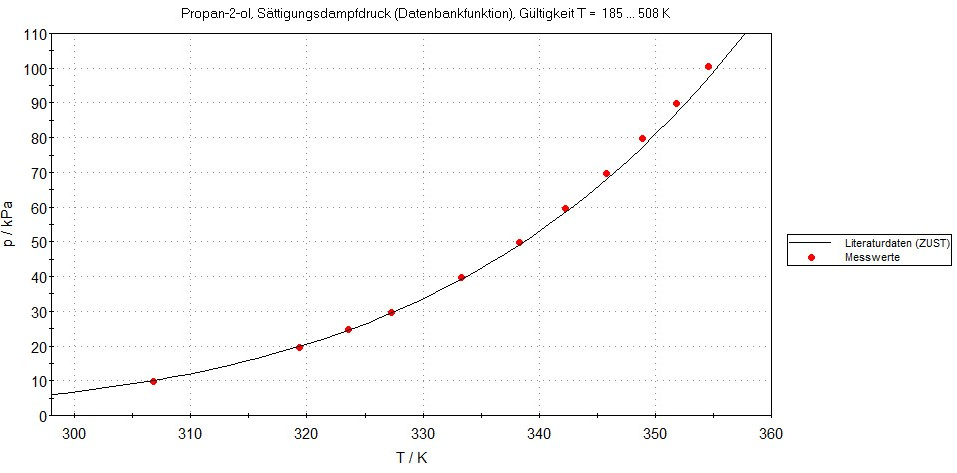
\includegraphics[width=1.0\textwidth]{img/literatur}
	\caption{Vergleich Messwerte und Literaturwerte}
	\label{fig:literatur}
\end{figure}
\FloatBarrier
%Ende

Um den Verlauf der Messdaten  modellhaft beschreiben zu können, ist es möglich die \textsc{Antoine}-Gleichung (Gl. \ref{gl:antoine}) zum Fitting der Messwerte zu nutzen. Daraus ergibt sich der in Abb. \ref{fig:antoine_fit} Graph der \textsc{Antoine}-Gleichung mit den Parametern aus Tab. \ref{tab:antoine_const} und den Messpunkten, welche experimentell bestimmt wurden. \linebreak 
Es wird der Druck in Abhängigkeit zur Temperatur dargestellt. Zu erkennen ist, dass mit steigendem Druck ebenfalls die gemessene Temperatur steigt.


\begin{figure}[h!]
	\centering
	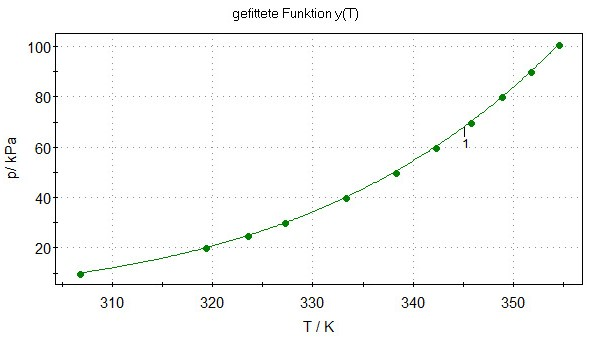
\includegraphics[width=1.0\textwidth]{img/antoine_fit}
	\caption{gefittete Messwerte mit \textsc{Antoine}-Parametern (siehe Tab. \ref{tab:antoine_const})}
	\label{fig:antoine_fit}
\end{figure}
\FloatBarrier
%Ende

% Table generated by Excel2LaTeX from sheet 'Daten'
\begin{table}[h!]
	\renewcommand*{\arraystretch}{1.2}
	\centering
	\caption{ \textsc{Antoine}-Parameter}
	\label{tab:antoine_const}
	\resizebox{14cm}{!}{
		\begin{tabulary}{1.2\textwidth}{C|C|C|C|C|C }
			\hline
			&\textbf{A} & \textbf{B} & \textbf{C}&\textbf{Restabweichung s}&\textbf{Temperaturbereich}\\
			\hline
			\textbf{Fitting}	&6,93& 1393,81&	201,38&\SI{3,18e-3}{}&$33,7$ bis \SI{81,5}{\celsius}\\
			\textbf{Literatur}&8,00&2010,33&252,64&-&$-25$ bis \SI{83}{\celsius}\\
			\hline
		\end{tabulary}
	}
\end{table}%
\FloatBarrier

Zur Berechnung der molaren Verdampfungsenthalpie wurde die Gleichung \ref{gl:verdamp} genutzt und ist unter der Gleichung \ref{gl:berechn_h} berechnet worden.


\begin{flalign}
\label{gl:berechn_h}
	\Delta^{\text{LV}} H_m &= -R* \frac{\ln\left(\frac{p_{s,T2}}{p_{s,T1}}\right)}{\frac{1}{T_2}-\frac{1}{T_1}}\\
	&= -\SI{8,314}{\joule \per \mol \per \kelvin}* \frac{\ln\left(\frac{\SI{10,00}{\kilo \pascal}}{\SI{100,66}{\kilo \pascal}}\right)}{\frac{1}{\SI{306,7}{\kelvin}}-\frac{1}{\SI{354,5}{\kelvin}}}\\
	&= \underline{\SI{43668,35}{\joule \per \mole}}
\end{flalign}

% Table generated by Excel2LaTeX from sheet 'Daten'
\begin{table}[h!]
	\renewcommand*{\arraystretch}{1.2}
	\centering
	\caption{Molare Verdampfungsenthalpie des Isopropanols}
	\label{tab:verdampf}
	%\resizebox{10.5cm}{!}{
	\begin{tabulary}{1.0\textwidth}{C|C }
		$\boldmath{\Delta^{\text{\textbf{LV}}} H_m(\SI{320}{\kelvin})} \left[\si{\joule \per \mol}\right]$ \textbf{Literatur}& $\boldmath{\Delta^{\text{\textbf{LV}}} H_m} \left[\si{ \joule \per \mol}\right]$ \textbf{Experiment}\\
		\hline
		43550& 43668		\\
		\hline
	\end{tabulary}
	%}
\end{table}%
\FloatBarrier

Der ermittelte Literaturwert über \textsc{ZUST} und die berechnete molare Verdampfungsenthalpie sind in Tab. \ref{tab:verdampf} gegenübergestellt. Es sind keine signifikanten Unterschiede festzustellen, welche auf eine fehlerhafte Berechnung des experimentellen Wertes hinweisen.

\begin{figure}[h!]
	\centering
	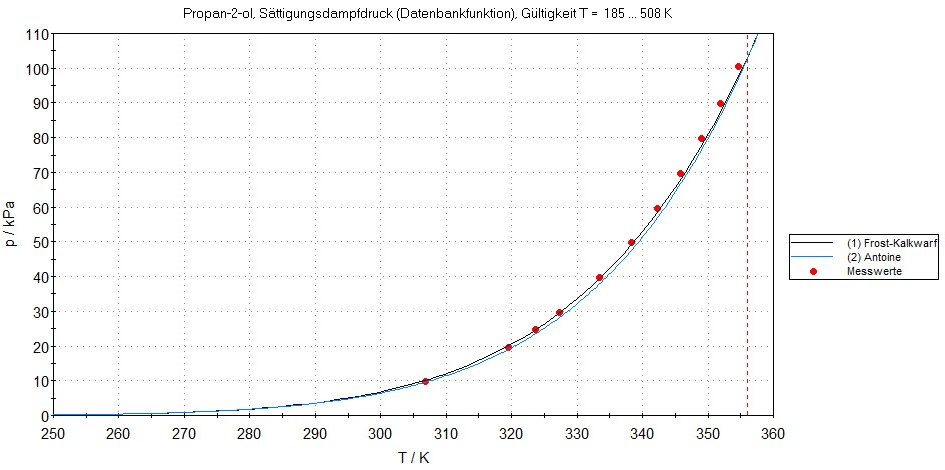
\includegraphics[width=1.0\textwidth]{img/vergleich}
	\caption{Vergleich des \textsc{Antoine}-Modells und des \textsc{Frost-Kalkwarf}-Modells für das Messwertfitting}
	\label{fig:vergleich}
\end{figure}
\FloatBarrier
%Ende
Ein weiteres mögliches Modell zum Fitting der Messdaten ist das \textsc{Frost-Kalkwarf}- Modell. In Abb. \ref{fig:vergleich} sind die Messpunkte und jeweils das Fitting über die \textsc{Frost-Kalkwarf}-Gleichung und die \textsc{Antoine}-Gleichung dargestellt. \\
Zu erkennen ist das \textsc{Frost-Kalkwarf}-Modell etwas besser die Messwerte erfasst, als das \textsc{Antoine}-Modell, welches bei den höhere Temperaturen deutlichere Abweichungen aufweist.
